\documentclass[UTF8, 12pt]{ctexart}
\usepackage{xcolor}
% 使用颜色
\definecolor{orange}{RGB}{255,127,0} 
\definecolor{violet}{RGB}{192,0,255} 
\definecolor{aqua}{RGB}{0,255,255} 
\usepackage{geometry}
\setcounter{tocdepth}{5}
\setcounter{secnumdepth}{5}
% 设置四级目录与标题
\geometry{papersize={21cm,29.7cm}}
% 默认大小为A4
\geometry{left=3.18cm,right=3.18cm,top=2.54cm,bottom=2.54cm}
% 默认页边距为1英尺与1.25英尺
\usepackage{indentfirst}
\setlength{\parindent}{2.45em}
% 首行缩进2个中文字符
\usepackage{amssymb}
% 因为所以与其他数学拓展
\usepackage{amsmath}
% 数学公式
\usepackage{setspace}
\renewcommand{\baselinestretch}{1.5}
% 1.5倍行距
\usepackage{pifont}
% 圆圈序号
\usepackage{tikz}
% 绘图
\usepackage{array}
% 设置表格行距
\usepackage[colorlinks,linkcolor=black,urlcolor=blue]{hyperref}
% 超链接
\author{Didnelpsun}
\title{函数与极限}
\date{}
\begin{document}
\renewcommand{\arraystretch}{1.5}
% 表格高1.5倍
\maketitle
\pagestyle{empty}
\thispagestyle{empty}
\tableofcontents
\thispagestyle{empty}
\newpage
\pagestyle{plain}
\setcounter{page}{1}
\section{映射与函数}
\subsection{邻域}
\subsubsection{一维}

邻域\textcolor{violet}{\textbf{定义:}}以点$x_0$为中心的任何开区间为点$x_0$的邻域,记为$U(x_0)$。

$\delta$邻域\textcolor{violet}{\textbf{定义:}}设$\delta$为一正数,则称开区间$(x_0-\delta,x_0+\delta)$为点$x_0$的$\delta$邻域,记作$U(x_0,\delta)$。$x_0$称为邻域的中心,$\delta$为邻域的半径。

去心$\delta$邻域就是去除$x_0$的$\delta$邻域,记为$\mathring{U}(x_0,\delta)$,左$\delta$邻域就是左侧的去心$\delta$邻域,记为$U^+(x_0,\delta)$,右$\delta$邻域就是右侧的去心$\delta$邻域,记为$U^-(x_0,\delta)$。

\subsubsection{二维}

邻域\textcolor{violet}{\textbf{定义:}}设点$P_0(x_0,y_0)$为$xOy$平面上的一点,$\delta$为某一个正数,与点$P_0(x_0,y_0)$的距离小于$\delta$的点$P(x,y)$的全体,称为点$P_0$的$\delta$邻域,记为$U(P_0,\delta)$。

同理可以得到去心$\delta$邻域的定义。

$\delta$邻域的几何意义:以$P_0(x_0,y_0)$为中心,以$\delta>0$为半径的圆内部所有的点。

函数的邻域就是一个区间,所以比如函数在某点的某邻域内有定义,就是说明函数在这个点的附近有定义,这个附近的距离没有必要说明。

\subsection{函数的概念}
\subsubsection{函数}
\begin{itemize}
    \item 函数即$y=f(x),x\in D$,x为自变量,y为因变量,D为定义域
    \item 一个x对应一个y,一个y可能对应多个x。
\end{itemize}
\subsubsection{反函数}
$y=f(x)$,定义域为$D$,值域为$R$,若对于每一个$y\in R$,必然存在$x\in D$使$y=f(x)$成立,则可以定义一个新函数$x=\psi(y)$,这个函数就是$y=f(x)$的\textbf{反函数},一般记作$x=f^{-1}(y)$,其定义域为$R$,值域为$D$,对于反函数,原来的函数称为\textbf{直接函数}。
\begin{enumerate}
    \item \textcolor{red}{严格单调}函数必然有反函数,即函数导数恒正或恒负必然有反函数。
    \item $x=f^{-1}(y)$与$y=f(x)$在同一坐标系中完全重合。
    \item $y=f^{-1}(x)$与$y=f(x)$关于$y=x$对称。
    \item $f[f^{-1}(x)]$或$f[\psi(x)]$变为x,称为湮灭。
\end{enumerate}
\subsubsection{复合函数}
设$y=f(u)$的定义域为$D_1$,函数$u=g(x)$在$D$上有定义且$g(D)\in D$,则由$y=f[g(x)],x\in D$确定的函数称为由函数$u=g(x)$和函数$y=f(u)$构成的复合函数,定义域为D,u为中间变量。

\textbf{例题:}设$f(x)=x^2$,$f[\psi(x)]=-x^2+2x+3$,且$\psi(x)\geqslant 0$,求$\psi(x)$以及定义域与值域。

广义化:$\because f(x)=x^2$,$\therefore f[\psi(x)]=\psi^2(x)=-x^2+2x+3$

又$\because\psi(x)\geqslant 0$, $\therefore\sqrt{\psi^2(x)}=\sqrt{-x^2+2x+3}=\psi(x)\geqslant 0$

$\therefore x\in[-1,3]$

$\therefore\dfrac{\rm{d}\psi(x)}{\rm{d}x}=(-x^2+2x+3)'=-2x+2=0$

$\therefore x=1$,驻点为1

又$\because(-x^2+2x+3)''=-2<0$

$\therefore$驻点为1时为最大值点,最大值为$\psi(1)=2$

又$\because\psi(-1)=\psi(3)=0$,$\therefore$最小值为0

$\therefore\psi(x)\in[0,2]$

\textcolor{orange}{注意}:$\sqrt{-x^2+2x+3}$为什么最值与$-x^2+2x+3$一致?

\textbf{例题:}求函数$y=f(x)=\ln(x+\sqrt{x^2+1})$的反函数$f^{-1}(x)$的表达式及其定义域

首先研究$f(x)$本身,因为$\ln(x)$的定义域必然要求大于0,而任意实数x都有下面不等式成立:

$x+\sqrt{x^2+1}>x+\vert x\vert \geqslant 0$,所以$x\in R$。

而研究其奇偶性:

$f(-x)=\ln(-x+\sqrt{x^2+1})=\ln(\dfrac{1}{\sqrt{x^2+1}+x})=-\ln(x+\sqrt{x^2+1})=-f(x)$

所以该函数为奇函数。

对其求单调性,即通过链式法则求导:

$\dfrac{\rm{d}y}{\rm{d}x}=\dfrac{1}{x+\sqrt{x^2+1}}\cdot (1+\dfrac{2x}{2\sqrt{x^2+1}})=\dfrac{1}{\sqrt{x^2+1}}>0$

所以该函数严格单调增。

然后求$y$的反函数:

$
    \begin{aligned}
        \because y & =\ln(x+\sqrt{x^2+1})     \\
        e^y        & =e^{\ln(x+\sqrt{x^2+1})} \\
                   & =x+\sqrt{x^2+1}
    \end{aligned}
$

$
    \begin{aligned}
        \because -y & =-\ln(x+\sqrt{x^2+1})          \\
                    & =\ln(\dfrac{1}{x+\sqrt{x^2+1}}) \\
                    & =\ln(\sqrt{x^2+1}-x)           \\
        e^{-y}      & =\sqrt{x^2+1}-x
    \end{aligned}
$

$
    \begin{aligned}
        \therefore e^y-e^{-y} & =2x                   \\
        x                     & =\dfrac{e^y-e^{-y}}{2}
    \end{aligned}
$

解出了用x表示y的函数表达$x=f^{-1}(y)$,即反函数,则$f^{-1}(x)=\dfrac{e^x-e^{-x}}{2}$

这种曲线为一种常见曲线:

\begin{itemize}
    \item $\dfrac{e^x-e^{-x}}{2}$:双曲正弦。
    \item $\dfrac{e^x+e^{-x}}{2}$:双曲余弦。(为一种悬链线)
    \item $\ln(x+\sqrt{x^2+1})$:反双曲正弦。
    \item $\ln(x+\sqrt{x^2-1})$:反双曲余弦。
\end{itemize}

\textbf{例题3:}设$
    f(x)=\left\{
    \begin{array}{lcl}
        \ln\sqrt{x}, &  & x\geqslant 1 \\
        2x-1,        &  & x< 1
    \end{array}
    \right.
$,求$f[f(x)]$

首先广义化:$
    f[f(x)]=\left\{
    \begin{array}{lcl}
        \ln\sqrt{f(x)}, &  & f(x)\geqslant 1 \\
        2f(x)-1,        &  & x<1
    \end{array}
    \right.
$

然后画图:\bigskip

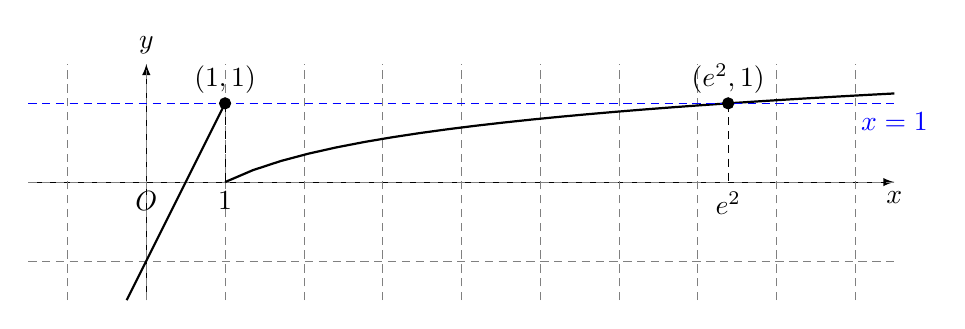
\begin{tikzpicture}[domain=-1:9.5]
    \draw[-latex](-1.5,0) -- (9.5,0) node[below]{$x$};
    \draw[-latex](0,-1.5) -- (0, 1.5) node[above]{$y$};
    \draw[very thin, gray, densely dashed](-1.5,1.5)grid(9.5,-1.5);
    \draw[black, thick](-0.25,-1.5) -- (1,1);
    \draw[black, thick,domain=1:9.5] plot (\x, {ln(sqrt(\x))});
    \draw[blue, densely dashed](-1.5,1) -- (9.5,1) node[below]{$x=1$};
    \filldraw[black] (1,1) circle (2pt) node[above]{$(1,1)$};
    \filldraw[black] (e^2,1) circle (2pt) node[above]{$(e^2,1)$};
    \draw[densely dashed](1,1) -- (1, 0) node[below]{$1$};
    \draw[densely dashed](e^2,1) -- (e^2,0) node[below]{$e^2$};
    \filldraw[black] (0,0) node[below]{$O$};
\end{tikzpicture}

所以将定义域分为三段:$[-\infty ,1],[1,e^2],[e^2, +\infty]$,然后根据不同定义域对应的不同函数再代回$f[f(x)]$:

$$
    f[f(x)]=\left\{
    \begin{array}{lcl}
        \ln\sqrt{\ln\sqrt{x}}, &  & x\geqslant e^2   \\
        \ln x-2,               &  & 1\geqslant x<e^2 \\
        4x-3,                  &  & x<1
    \end{array}
    \right.
$$

\subsection{函数的特性}

\subsubsection{有界性}

函数指明定义域区间才能讨论函数是否有界。

证明有界性:函数$f(x)$的定义域$D$,数集$I\in D$,如果存在某正数$M$,对于任一$x\in I$,有$\vert f(x)\vert\leqslant M$,则$f(x)$在$I$上有界,否则无界。

如果$f(x)\geqslant M$有下界,$f(x)\leqslant M$则有上界。

\subsubsection{单调性}

$y=f(x)\,x\in D$,如果$\forall x_1,x_2\in D$且$x_1<x_2$,有$f(x_1)<f(x_2)$,则函数在$D$上单调递增。反之则单调递减。

\bigskip

$\begin{matrix}
        \dfrac{\rm{d}y}{\rm{d}x}>0 & \Rightarrow & (x_1-x_2)[f(x_1)-f(x_2)]>0 & \Rightarrow & f(x)\nearrow \\
        \dfrac{\rm{d}y}{\rm{d}x}<0 & \Rightarrow & (x_1-x_2)[f(x_1)-f(x_2)]<0 & \Rightarrow & f(x)\searrow
    \end{matrix}
$

\subsubsection{奇偶性}

\begin{enumerate}
    \item 奇函数:关于原点对称,$f(-x)=-f(x)$。
    \item 偶函数:关于y轴对称,$f(-x)=f(x)$。
    \item 对于定义在$[-l,l]$上的任意函数$f(x)$,$F_1(x)=f(x)-f(-x)$必为奇函数,$F_2(x)=f(x)+f(-x)$必为偶函数。可以参考上面所说的双曲正弦与双曲余弦函数。
    \item 若奇函数在0处有定义,那么$f(0)=0$。
    \item 若偶函数在0处存在导数,那么$f'(0)=0$,即x=0,曲线必然水平,即导数为0。
    \item 若函数$y=f(x)$的函数关于直线$x=T$对称的充分必要条件是$f(x)=f(2T-x)/f(x+T)=f(x-T)$。(令$T-x=t$进行换元计算得到)
\end{enumerate}

\subsubsection{周期性}

$f(x+T)=f(x)$,其中T为周期。 \bigskip

\subsubsection{重要结论}

\begin{enumerate}
    \item 若$f(x)$为可导的偶函数,则$f'(x)$为奇函数。
    \item 若$f(x)$为可导的奇函数,则$f'(x)$为偶函数。
    \item 若$f(x)$为周期函数,则$f'(x)$也为周期函数且周期不变。
    \item 连续的奇函数的一切原函数都是偶函数。
    \item 连续的偶函数的原函数中仅有一个原函数是奇函数。
    \item 若连续函数$f(x)$以T为周期且$\int_{0}^{T}f(x)\rm{d}x=0$,则$f(x)$的一切原函数也以T为周期。
    \item 若$f(x)$在有限区间$(a,b)$中可导且$f'(x)$有界,则$f(x)$在$(a,b)$有界。(某一函数在固定区间内变化率是有界的,则变化范围是有界的)
\end{enumerate}

\textcolor{orange}{注意}:0和1处的函数定义应该注意。

如当a为0时:$f(b)-f(a)=f'(\xi )(b-a)=f(b)=bf'(\xi)$

如$f(x)>xf(1)$变形为$\dfrac{f(x)}{x}>f(1)$,辅助函数$F(x)=\dfrac{f(x)}{x}$

所以加减法警惕0,乘除法警惕1。

\section{数列的极限}

极限就是一个无限逼近某个值的过程。如$\dfrac{n}{n+1}$这个分式在$n$无限增大的时候会无限逼近1,这个1叫做极限值,所以写成$\lim\limits_{n\to\infty}\dfrac{n}{n+1}=1$。

所以从另一个方面更精确的指出一个数$N>0$,使得数列下标大于$N$的项与极限值之间的距离始终保持在$(0,\varepsilon)$之间,即$\dfrac{1}{n+1}<\varepsilon$,即$n>\dfrac{1}{\varepsilon}-1$,所以任意正数都能得到从$N>\dfrac{1}{\varepsilon}-1$项开始之后都有$\left\vert\dfrac{n}{n+1}-1\right\vert<\varepsilon$。

\subsection{定义}

通过定义可以证明极限。

\subsubsection{数列极限定义}

\textcolor{violet}{\textbf{定义:}}设$\{x_n\}$为一数列,若存在常数$a$,对于不论任意小的$\varepsilon>0$,总存在正整数$N$,使$n>N$时,$\vert x_n-a\vert<\varepsilon$恒成立,则常数$a$为数列$\{x_n\}$的极限,或$\{x_n\}$收敛于$a$,记为:$\lim\limits_{x\to\infty}x_n=a$或$x_n\to a(n\to\infty)$。

常用语言($\varepsilon-N$语言):$\lim\limits_{x\to\infty}x_n=a\Leftrightarrow\forall\varepsilon>0,\exists N\in N_+$,当$n>N$时,恒有$\vert x_n-a\vert<\varepsilon$。

如果不存在该数$a$,则称数列$x_n$发散。

即无论给出多么小的$\varepsilon$,总可以找到一项从该项之后函数值与极限值之间的差小于$\varepsilon$,即更接近这个极限值而不是其他任何值,所以该数列趋向于极限值。

\subsubsection{极限证明}

令$x_n$为通项,$a$为极限值,$\varepsilon$为任意正数。

\begin{enumerate}
    \item 写出$\vert x_n-a|<\varepsilon$。
    \item 反解出项数$n<g(\varepsilon)$。
    \item 取$N=[g(\varepsilon)]+1$,所以令$n>N$就可以证明。
\end{enumerate}

\textbf{例题:}用定义证明$\lim\limits_{x\to\infty}\left[1+\dfrac{(-1)^n}{n}\right]=1$

证明:

\ding{172}计算距离:$\left\vert 1+\dfrac{(-1)^n}{n}-1\right\vert=\left\vert\dfrac{(-1)^n}{n}\right\vert<\varepsilon$。

\ding{173}解得到:$\dfrac{1}{n}<\varepsilon$,反解为$n>\dfrac{1}{\varepsilon}$。

\ding{174}取整:$N=\left[\dfrac{1}{\varepsilon}\right]+1$。

$\therefore\forall\varepsilon>0$,当$n>N$时,就有$n>\dfrac{1}{\varepsilon}$,使得$\left\vert 1+\dfrac{(-1)^n}{n}-1\right\vert=\left\vert\dfrac{(-1)^n}{n}\right\vert<\varepsilon$。

$\therefore$证明完毕。

\textbf{例题:}用定义证明$\lim\limits_{n\to\infty}q^n=0$($q$为常数且$\vert q\vert<1$)。

证明:

\ding{172}$\vert q^n-0\vert<\varepsilon$。

\ding{173}$\vert q^n\vert<\varepsilon$,取对数进行反解$n\ln\vert q\vert<\ln\varepsilon$,又因为$\vert q\vert<1$,所以$\ln\vert q\vert<0$,所以得到$n>\dfrac{\ln\varepsilon}{\ln\vert q\vert}$。(若$\varepsilon>1$则$n$就是负数,这样条件必然成立)

\ding{174}取$N=\left[\dfrac{\ln\varepsilon}{\ln\vert q\vert}\right]+1$。

$\therefore$当$n>N$时,必然$n>\dfrac{\ln\varepsilon}{\ln\vert q\vert}$,有$\vert q^n-0\vert<\varepsilon$。

故$\lim\limits_{n\to\infty}q^n=0$。

\subsubsection{数列绝对值}

\textbf{例题:}证明若$\lim\limits_{x\to\infty}a_n=A$,则$\lim\limits_{x\to\infty}\vert a_n\vert=\vert A\vert$。

因为$\lim\limits_{n\to\infty}a_n=A\Leftrightarrow\forall\varepsilon>0,\exists N>0,\text{当}n>N$,恒有$\vert a_n-A\vert<\varepsilon$。

又由重要不等式$\vert\vert a\vert-\vert b\vert\vert\leqslant\vert a-b\vert$,所以$\vert\vert a_n-\vert A\vert\vert\leqslant\varepsilon$。

所以恒成立,证明完毕。

从这个题推出:$\lim\limits_{n\to\infty}a_n=0\Leftrightarrow\lim\limits_{n\to\infty}\vert a_n\vert=0$。所以如果我们以后需要证明某一数列极限为0,可以证明数列绝对值极限0,而数列绝对值绝对时大于等于0的,所以由夹逼准则,其中小的一头已经固定为0了,所以只用找另一个偏大的数列夹逼所证明数列就可以了。

\subsubsection{子数列}

\textcolor{violet}{\textbf{定义:}}从数列${a_n}:a_1,a_2,\cdots,a_n,\cdots$中选取无穷多项并按原来顺序组成的新数列就称为原数列的子列,记为$\{a_{n_k}\}:a_{n_1},a_{n_2},\cdots,a_{n_k},\cdots$。

若$n_k$分别取奇数和偶数,则得到奇数项数列与偶数项数列。

\textcolor{aqua}{\textbf{定理:}}若数列$\{a_n\}$收敛,则其任何子列$\{a_{n_k}\}$也收敛,且极限值相同。

所以对于其变式我们用到更多:

\begin{enumerate}
    \item 若一个数列$\{a_n\}$能找到一个发散的子列,那该数列发散。
    \item 若一个数列$\{a_n\}$能找到两个极限值不同的收敛子列,那么这个数列发散。
    \item 若一个数列$\{a_n\}$,则其奇数子列与偶数子列都收敛于同一个值。
\end{enumerate}

例如对于数列$\{(-1)^n\}$,能找到其奇数子列收敛于-1,偶数子列收敛于1,所以收敛值不同,原数列发散。

\subsection{性质}
\subsubsection{唯一性}

\textcolor{violet}{\textbf{定义:}}若数列$\{x_n\}$收敛于$a$,则$a$是唯一的。

证明:

设$\lim\limits_{n\to\infty}a_n=A$且$\lim\limits_{n\to\infty}a_n=B$且$A\neq B$。

不如设$A>B$。任意取$\varepsilon=\dfrac{A-B}{2}>0$。

$\because\lim\limits_{n\to\infty}a_n=A$

$\therefore\exists N_1>0$,当$n>N_1$时,$\vert a_n-A\vert<\dfrac{A-B}{2}$。

得到$\dfrac{A+B}{2}<a_n<\dfrac{3A-B}{2}$并设为式子一。

又$\because\lim\limits_{n\to\infty}a_n=B$

$\therefore\exists N_2>0$,当$n>N_2$时,$\vert a_n-B\vert<\dfrac{A-B}{2}$。

得到$\dfrac{3A-B}{2}<a_n<\dfrac{A+B}{2}$并设为式子二。

取$N=\max\{N_1,N_2\}$,当$n>N$时,式子一二同时成立,而$A\neq B$,则这两个式子不可能同时成立,矛盾。

同理$A<B$时也矛盾,所以$A\neq B$。

\subsubsection{有界性}

\textcolor{violet}{\textbf{定义:}}若数列$\{x_n\}$极限存在,则数列有界。

即$\lim\limits_{n\to\infty}a_n=A$,则存在$M>0$,使得$\vert a_n\vert\leqslant M$。

证明:

由极限定义,取$\varepsilon=1$。

$\because\lim\limits_{n\to\infty}a_n=A$

$\therefore\exists N>0$,当$n>N$时,$\vert a_n-A\vert<1$。

$\because\text{重要不等式}\,\vert\vert a_n\vert-\vert A\vert\vert\leqslant\vert a_n-A\vert$

$\therefore n>N$时,$\vert\vert a_n\vert-\vert A\vert\vert<1\Rightarrow\vert a_n\vert<1+\vert A\vert$

取$M=\max\{\vert a_1\vert,\vert a_2\vert,\cdots,\vert a_N\vert,1+\vert A\vert\}$

$\forall n$,有$\vert a_n\vert\leqslant M$

所以数列极限存在则数列有界。

但是数列有界不一定极限存在,如$1+(-1)^n$。

\subsubsection{保号性}

较重要。也称为脱帽法。

\textcolor{violet}{\textbf{定义:}}若数列$\{x_n\}$存在极限$\lim\limits_{n\to\infty}a_n=a\neq 0$,则存在正整数$N$,当$n>N$时$a_n$都与$a$同号。

简单来说,就是极限大于0,后面一部分数列大于0,极限小于0,后面一部分数列小于0。

推论,戴帽法:若数列$\{a_n\}$从某项开始$a_n\geqslant b$,且$\lim\limits_{n\to\infty}a_n=a$,则$a\geqslant b$。这里一定要带等号。

证明:

设$A>0$,取$\varepsilon=\dfrac{A}{2}>0$。

$\because\lim\limits_{n\to\infty}a_n=A$

$\therefore\exists N>0$,当$n>N$时,$\vert a_n-A\vert<\dfrac{A}{2}\Rightarrow a_n>\dfrac{A}{2}>0$

同理得证极限值小于0的情况。

\subsection{海涅定理(归结原则)}

设$f(x)$在$\mathring{U}(x_0,\delta)$内有定义,则$\lim\limits_{x\to x_0}f(x)=A$存在$\Leftrightarrow$对任何$\mathring{U}(x_0,\delta)$内以$x_0$为极限的数列$\{x_n\}(x_n\neq x_0)$,极限$\lim\limits_{n\to\infty}f(x_n)=A$存在。

海涅定理用来连接数列极限与函数极限。在极限存在下他们可以相互转换。

\textbf{例题:}求$\lim\limits_{n\to\infty}\left(n\tan\dfrac{1}{n}\right)^{n^2}$($n\in N^+$)。

$\because \lim\limits_{x\to 0}\left(\dfrac{\tan x}{x}\right)^{\frac{1}{x^2}}$

又$u^v=e^{v\ln u}$

$\therefore =e^{\lim\limits_{x\to 0}\frac{1}{x^2}\ln\frac{\tan x}{x}}$

又在$x\to 0$下$\ln (1+x)\sim x$,$\therefore \ln(1+g(x))\sim g(x),g(x)\to 0$。

而$\dfrac{\tan x}{x}$在$x\to 0$时趋于1,不满足趋于0的条件。

所以正好变形$\ln\left(1+\dfrac{\tan x}{x}-1\right)$。

$\therefore \ln\left(1+\dfrac{\tan x}{x}-1\right)\sim\dfrac{\tan x}{x}-1$,$\dfrac{\tan x}{x}-1\to 0$。

又根据泰勒展开$\tan x-x=x+\dfrac{x^3}{3}+o(x^3)-x-0\cdot x^3=\dfrac{x^3}{3}$。

$\therefore$ \bigskip

$
\begin{aligned}
    & e^{\lim\limits_{x\to 0}\frac{1}{x^2}\ln\frac{\tan x}{x}} \\
    & =e^{\lim\limits_{x\to 0}\frac{1}{x^2}\frac{\tan x-x}{x}} \\
    & =e^{\lim\limits_{x\to 0}\frac{1}{x^2}\cdot\frac{x^2}{3}} \\
    & = e^{\frac{1}{3}}
\end{aligned}
$

根据海涅定理:取$x=\dfrac{1}{n},n\to\infty$,$\lim\limits_{n\to\infty}\left(n\tan\dfrac{1}{n}\right)^{n^2}=e^{\frac{1}{3}}$。

\section{函数的极限}

\subsection{函数极限定义}

\subsubsection{极限定义}

设函数$f(x)$在点$x_0$的某一个去心邻域有定义,若存在常数$A$,对于任意给定的$\varepsilon>0$,总存在正数$\delta$,使得当$0<\vert x-x_0\vert<\delta$式,对应的函数值$f(x)$都满足不等式$\vert f(x)-A\vert <\varepsilon$,则$A$就是函数$f(x)$当$x\to x_0$时的极限,记作$\lim\limits_{x\to x_0}f(x)=A$或$f(x)\rightarrow A(x\rightarrow x_0)$。

写成$\varepsilon-\delta$语言:$\lim\limits_{x\to x_0}f(x)=A\Leftrightarrow\forall\varepsilon>0,\exists\delta>0,\text{当}0<\vert x-x_0\vert<\delta$时,有$\vert f(x)-A\vert\varepsilon$。

而对于趋向无穷时,写成$\varepsilon-X$语言:$\lim\limits_{x\to\infty}f(x)=A\Leftrightarrow\forall\varepsilon>0,\exists X>0,\text{当}\vert x\vert>X$时,有$\vert f(x)-A\vert<\varepsilon$。

\textcolor{orange}{注意:}这里的趋向分为六种:$x\to x_0$、$x\to x_0^+$、$x\to x_0^-$、$x\to\infty$、$x\to\infty^+$、$x\to\infty^-$。

\subsubsection{单侧极限}

当$x\to x_0^-$存在的极限称为左极限,当$x\to x_0^+$存在的极限称为右极限。

\subsubsection{函数极限存在条件}

函数存在的充要条件是:

\begin{enumerate}
    \item $\lim\limits_{x\to x_0}f(x)\Leftrightarrow\lim\limits_{x\to x_0^-}f(x)=\lim\limits_{x\to x_0^+}f(x)=A$。
    \item 函数脱帽法:$\lim\limits_{x\to x_0}f(x)\Leftrightarrow f(x)=A+\alpha(x),\lim\limits_{x\to x_0}\alpha(x)=0$,后面的$\alpha(x)$就是函数与极限值的误差。
\end{enumerate}

\subsubsection{极限情况总结}

\begin{center}
    \begin{tabular}{|c|c|c|c|c|}
        \hline
        过程 & $n\to\infty$ & $x\to\infty$ & $x\to+\infty$ & $x\to-\infty$ \\ \hline
        时刻 & \multicolumn{4}{c|}{$N$} \\ \hline
        从此时刻以后 & $n>N$ & $\vert x\vert>N$ & $x>N$ & $x<-N$ \\ \hline
        $f(x)$ & \multicolumn{4}{c|}{$\vert f(x)-A\vert<\varepsilon$} \\ 
        \hline
    \end{tabular}
\end{center}

\begin{center}
    \begin{tabular}{|c|c|c|c|}
        \hline
        过程 & $x\to x_0$ & $x\to x_0^+$ & $x\to x_0^-$ \\ \hline
        时刻 & \multicolumn{3}{c|}{$\delta$} \\ \hline
        从此时刻以后 & $0<\vert x-x_0\vert<\delta$ & $0<x-x_0<\delta$ & $-\delta<x-x_0<0$\\ \hline
        $f(x)$ & \multicolumn{3}{c|}{$\vert f(x)-A\vert<\varepsilon$} \\ 
        \hline
    \end{tabular}
\end{center}

\subsection{性质}

与数列极限性质类似,且任何$x$的趋向三个性质都是成立的。

\subsubsection{唯一性}

若极限存在,则极限唯一。

\textbf{例题:}设$a$为常数,$\lim\limits_{x\to 0}\left(\dfrac{e^{\frac{1}{x}}-\pi}{e^{\frac{2}{x}}+1}+a\cdot\arctan\dfrac{1}{x}\right)$存在,求出极限值。

因为求$x\to 0$,所以需要分两种情况讨论:

\bigskip

$
\begin{aligned}
    & \lim\limits_{x\to 0^+}\left(\dfrac{e^{\frac{1}{x}}-\pi}{e^{\frac{2}{x}}+1}+a\cdot\arctan\dfrac{1}{x}\right) \\
    & = \lim\limits_{x\to 0^+}\left(\dfrac{e^{\frac{1}{x}}-\pi}{e^{\frac{2}{x}}+1}\right)+\lim\limits_{x\to 0^+}\left(a\cdot\arctan\dfrac{1}{x}\right) \\
    & = \lim\limits_{x\to 0^+}\left(\dfrac{0\cdot\left(e^{\frac{2}{x}}\right)^2+e^{\frac{1}{x}}-\pi}{1\cdot\left(e^{\frac{2}{x}}\right)^2+1}\right)+a\cdot\dfrac{\pi}{2} \\
    & = a\cdot\dfrac{\pi}{2}
\end{aligned}
$

$
\begin{aligned}
    & \lim\limits_{x\to 0^-}\left(\dfrac{e^{\frac{1}{x}}-\pi}{e^{\frac{2}{x}}+1}+a\cdot\arctan\dfrac{1}{x}\right) \\
    & = -\pi+a\cdot\left(-\dfrac{\pi}{2}\right) \\
    & = -\pi-\dfrac{\pi}{2}\cdot a
\end{aligned}
$

因为极限值具有唯一性,所以$-\pi-\dfrac{\pi}{2}a=\dfrac{\pi}{2}a$,所以$a=-1$,极限值为$-\dfrac{\pi}{2}$。

\subsubsection{局部有界性}

若极限存在且为$A$,则存在正常数$M$和$\delta$,使得当$0<\vert x-x_0\vert<\delta$时,有$\vert f(x)\vert\leqslant M$。

\begin{enumerate}
    \item 极限存在是函数局部有界性的充分不必要条件。
    \item $f(x)$在$[a,b]$上连续,则$f(x)$在$[a,b]$上有界。
    \item 有限个有界函数与有界函数的和、差、积仍是有界函数。
    \item 若$f'(x)$在有限区间$(a,b)$内有界,则$f(x)$在该区间内有界。
\end{enumerate}

对于结论二,可以利用极限存在必然连续的概念,对$f(x)$在区间两端求极限从而证明有界。这里两端的极限不要求是一样的,因为两端不一样的极限表明该趋向点的极限值不存在,但是仍然有界。

证明结论四:

利用中值定理:$f(b)-f(a)=f'(\xi)(b-a)$。

令$x\in(a,b),x_0\in(a,b)$。其中这两个值不知道大小,只知道范围。

代入中值定理:$f(x)-f(x_0)=f'(\xi)(x-x_0)$

$
\begin{aligned}
    \vert f(x)\vert & =\vert f(x_0)+f'(\xi)(x-x_0)\vert \\
    & \leqslant\vert f(x_0)\vert+\vert f'(\xi)\vert\vert x-x_0\vert\text{ (重要绝对值不等式)} \\
    & \leqslant\vert f(x_0)\vert+K\cdot(b-a) \\
    & \leqslant M
\end{aligned}
$

\textbf{例题:}函数$f(x)=\dfrac{\vert x\vert\sin(x-2)}{x(x-1)(x-2)^2}$在哪个区间内有界()。

$A.(-1,0)$\qquad$B.(0,1)$\qquad$C.(1,2)$\qquad$D.(2,3)$

解:看选项,0,1,2出现次数较多,所以从$B$选项开始检查是否有界:

$\lim\limits_{x\to 0^-}\dfrac{\vert x\vert\sin(x-2)}{x(x-1)(x-2)^2}=(-1)\cdot\dfrac{-\sin 2}{(-1)\cdot 4}=-\dfrac{\sin 2}{4}$

所以趋于$0^-$的一段有界。

同理$\lim\limits_{x\to 0^+}\dfrac{\vert x\vert\sin(x-2)}{x(x-1)(x-2)^2}=\dfrac{\sin 2}{4}$。

所以趋于$0^+$的一段有界。

$\lim\limits_{x\to 1^-}\dfrac{\vert x\vert\sin(x-2)}{x(x-1)(x-2)^2}$中$(x-1)$为0且在分母位置,所以极限为$\infty$,无界。

所以$(0,1)$无界,$B$排除。

同理$\lim\limits_{x\to 1^+}\dfrac{\vert x\vert\sin(x-2)}{x(x-1)(x-2)^2}$也无穷大而无界。

所以$(1,2)$无界,$C$排除。

$\lim\limits_{x\to 2^+}\dfrac{\vert x\vert\sin(x-2)}{x(x-1)(x-2)^2}$中不管前面的项,而看到后面的$\dfrac{\sin(x-2)}{(x-2)^2}$。

因为$\lim\limits_{x\to 0}\dfrac{\sin x}{x}=1$,所以对于$\lim\limits_{x\to 2}\dfrac{\sin(x-2)}{(x-2)}=1$,所以下面还有一个$x-2$,所以还是为$\infty$。

所以$(2,3)$无界,$D$排除。

验证-1处是否有界:

$\lim\limits_{x\to -1}\dfrac{\vert x\vert\sin(x-2)}{x(x-1)(x-2)^2}=-\dfrac{\sin 3}{18}$。

所以该处有界,所以选$A$。

\subsubsection{局部保号性}

若极限存在,则存在常数$\delta>0$,使得当$0<\vert x-x_0\vert<\delta$时,$f(x)$与$A$同号。

简单来说,函数值在$x\to x_0$时函数值与极限值同号。

证明局部保号性:

首先根据极限存在定义:$\forall\varepsilon>0,\exists\delta>0,0<\vert x-x_0\vert<\delta$时,恒有$\vert f(x)-A\vert<\varepsilon$。

$\Rightarrow -\varepsilon<f(x)-A<\varepsilon$。

$\Rightarrow A-\varepsilon<f(x)<A+\varepsilon$。

任意取$\varepsilon=\dfrac{A}{2}>0\Rightarrow f(x)>A-\dfrac{A}{2}=\dfrac{A}{2}>0$。

证明完毕。

关于$\varepsilon$的取值问题,为什么不能取到令结果为负的值,因为请注意这个取值得到的区间并不是$f(x)$的范围,而是对$f(x)$所在区间的陈述,其是无尽逼近$A$的,所以取多大的区间都无所谓。

推论:若函数值在$x\to x_0$时都非负或非正,极限值为$A$,那么$A$与此时函数值同号。不能去除等号。

\bigskip

关于三个性质要注意自变量取值的双向性,所以需要留意下面几个函数:

\begin{enumerate}
    \item $\lim\limits_{x\to\infty}e^x$不存在,因为$\lim\limits_{x\to +\infty}e^x=+\infty$,$\lim\limits_{x\to -\infty}e^x=0$。
    \item $\lim\limits_{x\to 0}\dfrac{\sin x}{\vert x\vert}$不存在,因为$\lim\limits_{x\to 0^+}\dfrac{\sin x}{\vert x\vert}=1$,$\lim\limits_{x\to 0^-}\dfrac{\sin x}{\vert x\vert}=-1$。
    \item $\lim\limits_{x\to\infty}\arctan x$不存在,因为$\lim\limits_{x\to +\infty}\arctan x=\dfrac{\pi}{2}$,$\lim\limits_{x\to -\infty}\arctan x=-\dfrac{\pi}{2}$。
    \item $\lim\limits_{x\to 0}[x]$不存在,因为$\lim\limits_{x\to 0^+}[x]=0$,$\lim\limits_{x\to 0^-}[x]=-1$
\end{enumerate}

\section{无穷大与无穷小}

\subsection{无穷定义}

无穷小\textcolor{violet}{\textbf{定义:}}当$x\to x_0(\infty)$时,函数$f(x)$极限为0,就称$f(x)$为当$x\to x_0(\infty)$时的无穷小,记为:$\lim\limits_{x\to x_0(\infty)}f(x)=0$。

以0为极限的数列称为$n\to\infty$时的无穷小。

无穷小是变量,不能与很小的数相等。

零可以作为无穷小的唯一的数。

\textcolor{aqua}{\textbf{定理:}}$\lim f(x)=A\Leftrightarrow f(x)=A+o(x)$,其中$\lim o(x)=0$。

无穷大\textcolor{violet}{\textbf{定义:}}当$x\to x_0(\infty)$时,函数$\vert f(x)\vert$无限增大,就称$f(x)$为当$x\to x_0(\infty)$时的无穷大,记为:$\lim\limits_{x\to x_0(\infty)}f(x)=\infty$。

若$\lim\limits_{x\to x_0}f(x)=\infty$则$x=x_0$为$y=f(x)$的垂直渐进线。

若$\lim\limits_{x\to\infty}f(x)=a$则$y=a$为$y=f(x)$的水平渐进线。

\textcolor{aqua}{\textbf{定理:}}若同一极限过程中,$f(x)$为无穷大,则$\dfrac{1}{f(x)}$为无穷小,反之若$f(x)$为无穷小且不为0,则$\dfrac{1}{f(x)}$为无穷大。

\section{极限运算法则}

\begin{enumerate}
    \item 有限个无穷小的和是无穷小。
    \item 有界函数与无穷小的乘积是无穷小。
    \item 有限个无穷小的乘积是无穷小。
\end{enumerate}

\subsection{数列极限}

若$\lim\limits_{n\to\infty}x_n=a$,$\lim\limits_{n\to\infty}y_n=b$则:

\begin{enumerate}
    \item $\lim\limits_{n\to\infty}x_n\pm y_n=a\pm b$。
    \item $\lim\limits_{n\to\infty}(x_ny_n)=\lim\limits_{n\to\infty}x_n\lim\limits_{n\to\infty}y_n=ab$。
    \item $\lim\limits_{n\to\infty}\dfrac{x_n}{y_n}=\dfrac{\lim\limits_{n\to\infty}x_n}{\lim\limits_{n\to\infty}y_n}=\dfrac{a}{b}(b\neq 0)$。
\end{enumerate}

\textbf{例题:}若$\lim\limits_{n\to\infty}(a_n+b_n)=1$且$\lim\limits_{n\to\infty}(a_n-b_n)=3$,计算$\lim\limits_{n\to\infty}a_n$与$\lim\limits_{n\to\infty}b_n$。

首先是不能通过运算法则第一条将两个条件直接加减的,因为不能保证两个极限是否都存在。

所以必须先令$u_n=a_n+b_n$,$v_n=a_n-b_n$,所以$\lim\limits_{n\to\infty}u_n=1$,$\lim\limits_{n\to\infty}v_n=3$。

因为这两个极限都存在,所以可以进行运算。

相加得到$\lim\limits_{n\to\infty}(u_n+v_n)=2\lim\limits_{n\to\infty}a_n=4$。

所以得到$\lim\limits_{n\to\infty}a_n=2$。同理$\lim\limits_{n\to\infty}(u_n-v_n)$得到$\lim\limits_{n\to\infty}b_n=-1$。

\subsection{函数极限}

若$\lim f(x)=A$,$\lim g(x)=B$(即两个极限都存在),则

\begin{enumerate}
    \item $\lim[k\cdot f(x)\pm l\cdot g(x)]=k\lim f(x)\pm l\cdot g(x)=kA\pm lB$,其中$kl$为常数。
    \item $\lim[f(x)\cdot g(x)]=\lim f(x)\cdot\lim g(x)=A\cdot B$
    \item $\lim[f(x)]^n=[\lim f(x)]^n$,其中$n$为正整数。
    \item $\lim\dfrac{f(x)}{g(x)}=\dfrac{\lim f(x)}{\lim g(x)}=\dfrac{A}{B}(B\neq 0)$。
    \item $\lim\limits_{x\to\infty}\dfrac{a_nx^n+a_{n-1}x^{n-1}+\cdots+a_1x+a_0}{b_mx^m+\cdots+b_{m-1}x^{m-1}+\cdots+b_1x+b_0}=\left\{
        \begin{array}{lcl}
            \dfrac{a_n}{b_m}, & & n=m \\
            0, & & n<m \\
            \infty, & & n>m
        \end{array}
    \right.$
    \item 若$f(x)\geqslant g(x)$,则$A\geqslant B$。
    \item 若$y=f[g(x)]$由$y=f(u)$与$u=g(x)$复合而成,且$\lim\limits_{x\to x_0}g(x)=u_0$且$\lim\limits_{u\to u_0}f(u)=a$,当$x\in\mathring{U}(x_0,\delta_0)$时,$g(x)\neq u_0$,则$\lim\limits_{x\to x_0}f[g(x)]=a$。 
\end{enumerate}

对于结论7必须\textcolor{orange}{注意}$g(x)\neq u_0$。

假设$f(u)=\dfrac{u^2-1}{u-1}$,所以这个$f(x)$在$x=1$处应无定义。但是这并不影响$\lim\limits_{u\to 1}f(u)=2$。

假设$g(x)=\left\{
    \begin{array}{lcl}
        1+x, & & x<0 \\
        1, & & x>0
    \end{array}
\right.$。

则$\lim\limits_{x\to 0}g(x)=1$,所以$\lim\limits_{x\to 0}f[g(x)]=2?$。

答案是不,因为当$x>0$时,$u=g(x)=1$,而$1$在$g(x)$中是无定义的,所以复合函数当$x>0$时无定义,从而在$0$处极限不存在。

\subsection{存在与不存在运算关系}

\begin{enumerate}
    \item 存在与不存在的和差一定为不存在。
    \item 不存在与不存在的和差不一定存在,如$\sin\dfrac{1}{x}+\sin\dfrac{1}{x}$与$\sin\dfrac{1}{x}+\left(-\sin\dfrac{1}{x}\right)$。
    \item 存在与不存在的乘积不一定存在,如$x\sin\dfrac{1}{x}$与$1\cdot\sin\dfrac{1}{x}$。
    \item 不存在与不存在的乘积不一定存在,如$\dfrac{1}{x}\cdot\dfrac{1}{x}$与$(-1)^n\cdot(-1)^n$。
\end{enumerate}

\section{极限存在准则与两个重要极限}

\subsection{夹逼准则}

\subsubsection{数列的夹逼准则}

\begin{enumerate}
    \item $y_n\leqslant x_n\leqslant z_n(n=1,2,3,\cdots)$。
    \item $\lim\limits_{n\to\infty}y_n=a,\lim\limits_{n\to\infty}z_n=a$。
    \item 则$\lim\limits_{n\to\infty}x_n=a$。
\end{enumerate}

证明:

由于$\lim\limits_{n\to\infty}y_n=a,\lim\limits_{n\to\infty}z_n=a$。

则$\forall\varepsilon>0$,$\exists N$,当$n>N$时,$\vert y_n<\varepsilon$,$\vert z_n<\varepsilon$。

$\therefore a-\varepsilon<y_n<a+\varepsilon$,$a-\varepsilon<z_n<a+\varepsilon$。

$\therefore a-\varepsilon<y_n\leqslant x_n\leqslant z_n<a+\varepsilon$。

$\therefore\vert x_n-a\vert<\varepsilon$。

\textbf{例题:}求极限$\lim\limits_{n\to\infty}\left(\dfrac{n}{n^2+1}+\dfrac{n}{n^2+2}+\cdots+\dfrac{n}{n^2+n}\right)$。

使用夹逼准则:$\dfrac{n^2}{n^2+n}<\sum_{i=1}^n\dfrac{n}{n^2+i}<\dfrac{n^2}{n^2+1}$。

又$\lim\limits_{n\to\infty}\dfrac{n^2}{n^2+1}=\lim\limits_{n\to\infty}\dfrac{n^2/n^2}{n^2/n^2+1/n^2}=\lim\limits_{n\to\infty}\dfrac{1}{1+\dfrac{1}{n^2}}=1$。

且$\lim\limits_{n\to\infty}\dfrac{n^2}{n^2+n}=\lim\limits_{n\to\infty}\dfrac{1}{1+\dfrac{1}{n}}=1$。

由夹逼准则,原式的极限为1。

数列的夹逼准则下不等式的证明往往要使用到放缩法,对于分式的放缩主要在于分母的放缩,不变分子,分母变小原式变大,分母变大原式变小。然后分子分母除以最高项得到逼向0的极限。

\subsubsection{函数的夹逼准则}

\begin{enumerate}
    \item $x\in\mathring{U}(x_0,\delta)$时$g(x)\leqslant f(x)\leqslant h(x)$。
    \item $\lim g(x)=A$且$\lim h(x)=A$。
    \item 则$\lim f(x)=A$。
\end{enumerate}

\textcolor{orange}{注意:}两函数差值极限为0不代表两函数极限相同,也不能保证中间的$f(x)$的极限存在。

\textbf{例题:}求$\lim\limits_x\to+\infty(2+\sin x)^{\frac{1}{x}}$。

$\because \sin x\in[-1,1]$,$\therefore 1\leqslant 2+\sin x\leqslant 3$。

$\therefore 1^{\frac{1}{x}}\leqslant\left(2+\sin x\right)^{\frac{1}{x}}\leqslant 3^{\frac{1}{x}}$。

而当$x\to+\infty$时两边的极限都为$1$,则由夹逼定理$\lim\limits_x\to+\infty(2+\sin x)^{\frac{1}{x}}=1$。

\subsection{单调有界准则}

也称为魏尔施特拉斯准则,该部分对于数列而言最重要。

对于函数而言也有单调有界准则,但是很少用到。

\textcolor{violet}{\textbf{定义:}}单调有界数列必有极限,即若$\{x_n\}$单调增加(减少)且有上界(下界),则极限存在。

该部分需要证明两个地方:

\begin{enumerate}
    \item 数列单调:$x_{n+1}-x_n$与0的关系,或$\dfrac{x_{n+1}}{x_n}$与1的关系。
    \item 有界:$\vert x_n\vert\leqslant M$是否存在。
\end{enumerate}

见到\textcolor{orange}{递推式(迭代式)}$a_{n+1}=f(a_n)$,一般都要用单调有界准则。单调性通过减或除进行计算,有界性通过不等式来计算。

\textbf{例题:}已知$a_1=a>0$,证明$a_{n+1}=\dfrac{1}{2}\left(a_n+\dfrac{2}{a_n}\right)$的极限存在并求出。

$\because a_1=a>0$,且递推式中没有负数与减的操作,所以$a_n>0$。

由重要不等式$\dfrac{a+b}{2}\geqslant\sqrt{ab}$,所以$a_{n+1}=\dfrac{1}{2}\left(a_n+\dfrac{2}{a_n}\right)\geqslant\sqrt{a_n\cdot\dfrac{2}{a_n}})=\sqrt{2}$

$\therefore$数列$\{a_n\}$有下界$\sqrt{2}$。

又$a_{n+1}-a_n=\dfrac{2-a_n^2}{2a_n}$,且由上面证明已知$a_n^2\geqslant\sqrt{2}$,所以该式子小于等于0。

$\therefore a_{n+1}\leqslant a_n$,得到数列单调减少。

由单调有界准则,$\lim\limits_{n\to\infty}a_n$存在并记为$A$。

将$A$代入递推式并两边求极限:$A=\dfrac{1}{2}(A+\dfrac{2}{A})$,得到$A=\pm\sqrt{2}$。

又因为保号性,数列下界为$\sqrt{2}$,所以$A=\sqrt{2}$。

\textbf{例题:}求证$x_{n+1}=\sin x_n$极限存在,$0<x_1<\pi$。

由三角函数中的不等式$\sin x<x$。

\ding{172}当$n=1$,$\because 0<x_1<\pi$,$\therefore 0<\sin x_1<1$,$\therefore 0<x_2=sin x_1<x<\pi$。

\ding{173}假设$0<x_n=\sin x_{n-1}<\pi$。

\ding{174}$\therefore 0<x_{n+1}=\sin x_n<x_n<\pi$。

\ding{175}故$\{x_n\}\searrow$且有下界0。

$\therefore\lim\limits_{n\to\infty}x_n$存在,并记为$A$。

对两边取极限:$A=\sin A$,所以$A=0$。

$\therefore\lim\limits_{n\to\infty}x_n=0$。

\textbf{例题:}证明$a_n=\dfrac{1}{1^2}+\dfrac{1}{2^2}+\cdots+\dfrac{1}{n^2}$存在极限。

因为是递推式,所以一般使用单调有界准则。

\ding{172}$a_{n+1}=\dfrac{1}{1^2}+\dfrac{1}{2^2}+\cdots+\dfrac{1}{n^2}+\dfrac{1}{(n+1)^2}$。

$\Rightarrow a_{n+1}-a_n=\dfrac{1}{(n+2)^2}>0\Rightarrow\{a_n\}\nearrow$

$
\begin{aligned}
    \text{\ding{173}}a_n & =\dfrac{1}{1\cdot 1}+\dfrac{1}{2\cdot 2}+\cdots+\dfrac{1}{n\cdot n} \\
    & \text{裂项相消} \\
    < & 1+\dfrac{1}{1\cdot 2}+\cdots+\dfrac{1}{(n-1)\cdot(n)} \\
    = & 1+(1-\dfrac{1}{2})+(\dfrac{1}{2}-\dfrac{1}{3})+\cdots+(\dfrac{1}{n-1}-\dfrac{1}{n}) \\
    = & 2-\dfrac{1}{n} \\
    < & 2 \text{ (上界)}
\end{aligned}
$

单调增且有上界,所以必然有极限。

\subsection{\texorpdfstring{$\lim\limits_{x\to 0}\dfrac{\sin x}{x}=1$}{}}

证明:

当$x\to 0$时$x\in[0,\dfrac{\pi}{2}]$。

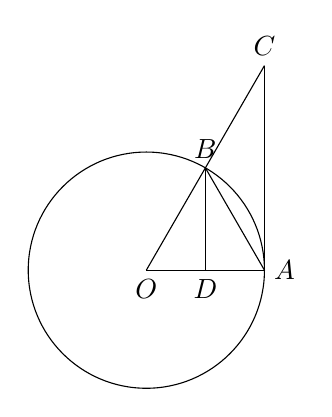
\begin{tikzpicture}[scale=1.5]
    \draw (0,0) circle (1);
    \filldraw[black] (0,0) node[below]{$O$};
    \draw[black](0,0) -- (1,0) node[right]{$A$};
    \draw[black](0,0) -- (1/2,{sqrt(3)/2}) node[above]{$B$};
    \draw[black](1/2,{sqrt(3)/2}) -- (1/2,0) node[below]{$D$};
    \draw[black](1,0) -- (1,{sqrt(3)}) node[above]{$C$};
    \draw[black](1,0) -- (1/2,{sqrt(3)/2});
    \draw[black](1,{sqrt(3)}) -- (1/2,{sqrt(3)/2});
\end{tikzpicture}

设$\angle AOB$的弧度为$x$,圆$O$的半径为$1$,则$OD=\sin x$。

则$S_\vartriangle AOB=\dfrac{\sin x}{2}$。根据扇形面积公式:$S_{\text{扇形}}AOB=\dfrac{x}{2}$。

又$\because CA=\tan x$,则$S_\vartriangle AOC=\dfrac{\tan x}{2}$。

根据图,在$x\in[0,\dfrac{\pi}{2}]$,$\sin x<x<\tan x$。

$\therefore 1<\dfrac{x}{\sin x}<\dfrac{1}{\cos x}\Rightarrow\cos x<\dfrac{\sin x}{x}<1$。

$\therefore 0<1-\dfrac{\sin x}{x}<1-\cos x=2\sin^2\dfrac{x}{2}\leqslant 2\left(\dfrac{x}{2}\right)^2$。

根据夹逼定理,$\lim\limits_{x\to 0}2\left(\dfrac{x}{2}\right)^2=0\Rightarrow\lim\limits_{x\to 0}1-\dfrac{\sin x}{x}=0$。

$\therefore\lim\limits_{x\to 0}\dfrac{\sin x}{x}=1$。

从而$\lim\limits_{\Delta\to 0}\dfrac{\sin\Delta}{\Delta}=1(\Delta\neq 0)$。

\subsection{\texorpdfstring{$\lim\limits_{x\to\infty}\left(1+\dfrac{1}{x}\right)^x=e$}{}}

书上通过数列进行单调有界定理证明极限存在性。

证明:

$
\begin{aligned}
    & \lim\limits_{x\to\infty}\left(1+\dfrac{1}{x}\right)^x \\
    & =\lim\limits_{x\to\infty}e^{\ln(1+\frac{1}{x})^x} \\
    & =\lim\limits_{x\to\infty}e^{x\ln(1+\frac{1}{x})} \\
    & =e^{\lim\limits_{x\to\infty}x\ln(1+\frac{1}{x})} \\
    & =e^{\lim\limits_{x\to\infty}\frac{\ln(1+\frac{1}{x})}{\frac{1}{x}}} \\
    & =e^{\lim\limits_{x\to\infty}\frac{\left(\frac{1}{1+\frac{1}{x}}\right)\cdot\left(-\frac{1}{x^2}\right)}{-\frac{1}{x^2}}} \\
    & =e^{\lim\limits_{x\to\infty}\frac{1}{1+x}} \\
    & =e
\end{aligned}
$

从而$\lim\limits_{\Delta\to\infty}\left(1+\dfrac{1}{\Delta}\right)^\Delta=e$与$\lim\limits_{\Delta\to 0}\left(1+\Delta\right)^{\frac{1}{\Delta}}=e(\Delta\neq 0)$。

\section{无穷小的比较}

\subsection{无穷小量}

\textcolor{violet}{\textbf{定义:}}若$\lim\limits_{x\to x_0}f(x)=0$,则称$f(x)$为当$x\to x_0$时的无穷小量。

\subsection{无穷小的比较}

设在自变量同一变化过程中,$\lim\alpha(x)=0$,$\lim\beta(x)=0$,且$\beta(x)\neq 0$,则:

\begin{enumerate}
    \item 若$\lim\dfrac{\alpha(x)}{\beta(x)}=0$,则$\alpha(x)$是比$\beta(x)$高阶的无穷小,记为$\alpha(x)=o(\beta(x))$。
    \item 若$\lim\dfrac{\alpha(x)}{\beta(x)}=\infty$,则$\alpha(x)$是比$\beta(x)$低阶的无穷小。
    \item 若$\lim\dfrac{\alpha(x)}{\beta(x)}=c\neq 0$,则$\alpha(x)$与$\beta(x)$是同阶无穷小。
    \item 若$\lim\dfrac{\alpha(x)}{\beta(x)}=1$,则$\alpha(x)$与$\beta(x)$是等价无穷小,记为$\alpha(x)\sim\beta(x)$。
    \item 若$\lim\dfrac{\alpha(x)}{[\beta(x)]^k}=c\neq 0$,则$\alpha(x)$是$\beta(x)$的$k$阶无穷小。
\end{enumerate}

\textcolor{aqua}{\textbf{定理:}}$\alpha(x)\sim\beta(x)$的充要条件是$\alpha(x)=\beta(x)+o(\beta(x))$。

\textcolor{orange}{注意:}并不是任意无穷小都可以比阶。如$\lim\limits_{x\to 0}\dfrac{x\sin\dfrac{1}{x}}{x^2}$就因为得到函数振荡而无法得到极限。

\textbf{例题:}证明当$x\to 0$时,$\sqrt[n]{1+x}-1\sim\dfrac{1}{n}x$。

证明$\sqrt[n]{1+x}-1\sim\dfrac{1}{n}x$就是证明$\lim\limits_{x\to 0}\dfrac{\sqrt[n]{1+x}-1}{x}\sim\dfrac{1}{n}$。

令$\sqrt[n]{1+x}-1=t$,则$1+x=(1+t)^n$,则$x=(1+t)^n-1$。

利用二项式展开:$=\lim\limits_{t\to 0}\dfrac{t}{nt+\dfrac{n(n-1)}{2}t^2+\cdots}=\dfrac{1}{n}$。

\subsection{无穷小运算}

设$m$,$n$为正整数:

\begin{enumerate}
    \item $o(x^m)\pm o(x^n)=o(x^l),l=\min{m,n}$(加减法低阶吸收高阶)。
    \item $o(x^m)\cdot o(x^n)=o(x^{m+n}),x^m\cdot o(x^n)=o(x^{m+n})$(乘法累加)。
    \item $o(x^m)=o(k\cdot x^m)=k\cdot o(x^m)$,$k\neq 0$且为常数(非零常数相乘不影响阶数)。
\end{enumerate}

\subsection{常用等价无穷小}

\textcolor{aqua}{\textbf{定理:}}若$\alpha\sim\alpha_1$,$\beta\sim\beta_1$,则$\lim\dfrac{\alpha}{\beta}=\lim\dfrac{\alpha_1}{\beta}=\lim\dfrac{\alpha}{\beta_1}=\lim\dfrac{\alpha_1}{\beta_1}$。

所以可以使用等价无穷小替换对应式子,这些等价无穷小都是使用泰勒展开得到的。

\textcolor{red}{警告:}一般只有所替换的式子为乘除的整个因子才能替换,加减一般都不能替换,如$x-\sin x\sim\dfrac{1}{6}x^3$。

$x\to 0$:

\begin{enumerate}
    \item $\sin x\sim x$。
    \item $\tan x\sim x$。
    \item $\arcsin x\sim x$。
    \item $\arctan x\sim x$。
    \item $\ln(1+x)\sim x$。
    \item $e^x-1\sim x$。
    \item $a^x-1\sim x\ln a$。
    \item $1-\cos x\sim\dfrac{1}{2}x^2$。
    \item $(1+x)^a-1\sim ax$。
\end{enumerate}

还有$e^{\sin x}-e^x\sim\sin x-x\sim-\dfrac{1}{6}x^3$。

其中$a\cdot x\ln x$当$x\to 0$的极限必然为0。

\section{函数连续性与间断点}

函数的连续与间断是逐点的概念。

\subsection{连续定义}

若函数$f(x)$在点$x_0$的某一邻域内有定义,且有$\lim\limits_{x\to x_0}f(x)=f(x_0)$或$\lim\limits_{\Delta x\to 0}\Delta y=0$,则称函数$f(x)$在点$x_0$处连续。

极限值等于函数值,则该点连续。

\subsection{间断定义}

讨论间断只看两类点:分段函数分段点,无定义点。

若函数$f(x)$在点$x_0$的某一去心邻域内有定义,且有$\lim\limits_{x\to x_0}f(x)\neq f(x_0)$,则称函数$f(x)$在点$x_0$处间断。

极限值不等于函数值,则该点间断。

\subsection{间断点分类}

\subsubsection{可去间断点(可补间断点)}

若$\lim\limits_{x\to x_0}f(x)=A\neq f(x_0)$(甚至可以没有定义)。

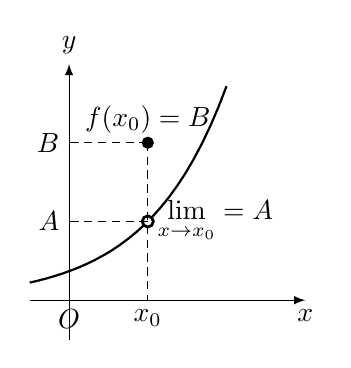
\begin{tikzpicture}
    \draw[-latex](-0.5,0) -- (3,0) node[below]{$x$};
    \draw[-latex](0,-0.5) -- (0,3) node[above]{$y$};
    \filldraw[black] (0,0) node[below]{$O$};
    \draw[black, thick, domain=-0.5:2] plot (\x,{pow(e,\x-1)});
    \filldraw[white, draw=black, line width=1pt] (1,1) circle (2pt);
    \draw[black, densely dashed](1,2) -- (0,2) node[left]{$B$};
    \draw[black, densely dashed](1,1) -- (0,1) node[left]{$A$};
    \draw[black, densely dashed](1,2) -- (1,0) node[below]{$x_0$};
    \filldraw[black] (1,2) circle (2pt) node[above]{$f(x_0)=B$};
    \filldraw[black] (1,1) node[right]{$\lim\limits_{x\to x_0}=A$};
\end{tikzpicture}

\subsubsection{跳跃间断点}

若$\lim\limits_{x\to x_0^-}f(x)$与$\lim\limits_{x\to x_0^+}$都存在,但是$\lim\limits_{x\to x_0^-}f(x)\neq\lim\limits_{x\to x_0^+}$。

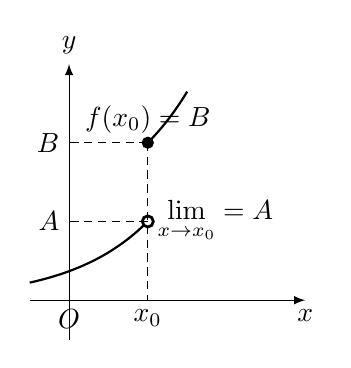
\begin{tikzpicture}
    \draw[-latex](-0.5,0) -- (3,0) node[below]{$x$};
    \draw[-latex](0,-0.5) -- (0,3) node[above]{$y$};
    \filldraw[black] (0,0) node[below]{$O$};
    \draw[black, thick, domain=-0.5:1] plot (\x,{pow(e,\x-1)});
    \draw[black, thick, domain=1:1.5] plot (\x,{pow(e,\x-1)+1});
    \filldraw[white, draw=black, line width=1pt] (1,1) circle (2pt);
    \draw[black, densely dashed](1,2) -- (0,2) node[left]{$B$};
    \draw[black, densely dashed](1,1) -- (0,1) node[left]{$A$};
    \draw[black, densely dashed](1,2) -- (1,0) node[below]{$x_0$};
    \filldraw[black] (1,2) circle (2pt) node[above]{$f(x_0)=B$};
    \filldraw[black] (1,1) node[right]{$\lim\limits_{x\to x_0}=A$};
\end{tikzpicture}

可去间断点与跳跃间断点的左右极限都存在的点都称为第一类间断点。

\subsubsection{无穷间断点}

若$\lim\limits_{x\to x_0}f(x)=\infty$,或至少一个方向为无穷大(定义分歧)。如$y=\dfrac{1}{x}$在$x=0$处为无穷间断点。

\begin{tikzpicture}
    \draw[-latex](-2,0) -- (2,0) node[below]{$x$};
    \draw[-latex](0,-2) -- (0,2) node[above]{$y$};
    \filldraw[black] (0,0) node[below]{$O$};
    \draw[black, thick, domain=0.5:2] plot (\x,{pow(\x,-1)});
    \draw[black, thick, domain=-2:-0.5] plot (\x,{pow(\x,-1)});
\end{tikzpicture}

\subsubsection{振荡间断点}

若$\lim\limits_{x\to x_0}f(x)$为振荡不存在。如$\lim\limits_{x\to 0}\sin\dfrac{1}{x}$的$x=0$就是振荡间断点。

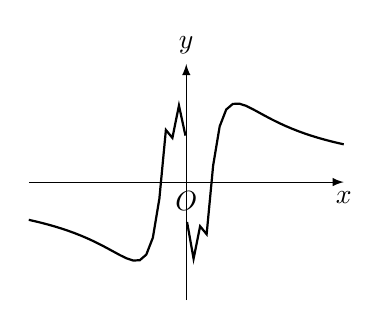
\begin{tikzpicture}
    \draw[-latex](-2,0) -- (2,0) node[below]{$x$};
    \draw[-latex](0,-1.5) -- (0,1.5) node[above]{$y$};
    \filldraw[black] (0,0) node[below]{$O$};
    \draw[black, thick, domain=0.01:2] plot (\x,{sin(pow(\x,-1) r)});
    \draw[black, thick, domain=-2:-0.01] plot (\x,{sin(pow(\x,-1) r)});
\end{tikzpicture}

无穷间断点与振荡间断点的左右极限都不存在的点都是第二类间断点。

\textcolor{orange}{注意:}两侧邻域都有定义才能讨论间断点问题。

\textbf{例题:}若$f(x)=\left\{
    \begin{array}{lcl}
        2x+a, & & x\leqslant 0 \\
        e^x(\sin x+\cos x), & & x>0
    \end{array} \right.
$在$(-\infty,+\infty)$内连续,求$a$。

因为连续,所以$f(0)=\lim\limits_{x\to 0^+}f(x)=\lim\limits_{x\to 0^-}f(x)$。

$\therefore a=1$。

\textbf{例题:}若函数$f(x)=\dfrac{\ln\vert x\vert}{\vert x-1\vert}\sin x$,则x的间断点类型是?

由式子的分式部分可知有两个无定义的间断点:$x=0$,$x=1$。

$\lim\limits_{x\to 1}f(x)=\lim\limits_{x\to 1}\dfrac{x-1}{\vert x-1\vert}\sin x=\left\{
    \begin{array}{lcl}
        x\to 1^+ & \rightarrow & \sin 1 \\
        x\to 1^- & \rightarrow & -\sin 1
    \end{array} \right.
$。

所以$x=1$跳跃间断点。

$\lim\limits_{x\to 0}f(x)=\lim\limits_{x\to 0}\ln\vert x\vert\cdot\sin x=\lim\limits_{x\to 0}x\ln\vert x\vert=0$。

而$x=0$未定义,所以其为可去间断点。

\subsection{函数连续性}

\subsubsection{连续函数四则运算的连续性}

若两个函数在某点连续,则这两个函数的和差积商在该点都连续。

\subsubsection{反函数的连续性}

若函数在定义域是严格单调的函数,则其反函数在其原值域上也是连续的。

\subsubsection{复合函数的连续性}

若$y=f(g(x))$由$y=f(u)$与$u=g(x)$复合而成,若$g(x)$在$x_0$处连续,$f(u)$在$u_0$处连续,且$u_0=g(x_0)$,则$f(g(x))$在$x_0$处连续。

\subsubsection{初等函数的连续性}

基本初等函数在定义域上是连续的。

初等函数在定义区间上是连续的。

定义区间是定义域的子集。

\section{闭区间上连续函数的性质}

设$f(x)$在区间$[a,b]$上连续,则:

\begin{enumerate}
    \item 最大最小值定理:$f(x)$在$[a,b]$上必有最大值和最小值。
    \item 有界性定理:$f(x)$在$[a,b]$上必有界。
    \item 零点定理:若$f(a)f(b)<0$,则$\exists\,\xi\in[a,b]$使得$f(\xi)=0$。
    \item 介值定理:若$f(a)\neq f(b)$,$\mu$为介于$f(a)$与$f(b)$之间的任何值,那么至少存在$\xi\in[a,b]$使得$f(\xi)=\mu$。
\end{enumerate}

\textbf{例题:}证明方程$x=a\sin x+b(a>0,b>0)$中至少有一个正根,并且不超过$a+b$。

令$f(x)=x-a\sin x-b$,其中$f(0)=-b<0$,$f(a+b)=a+b=a\sin(a+b)-b=a[1-\sin(a+b)]\geqslant 0$。

若$\sin(a+b)=1$,则根为$a$,结论成立。

若$\sin(a+b)<1$,$\because f(a+b)\cdot f(0)<0$根据零点定理$\exists\,\xi\in[0,a+b]$使得$f(\xi)=0$,从而得证。


\end{document}
